% ---------------------------------------------------------------
%  EnergyTech / معهد الطاقة  --  Chapter 04, version B
%  Questions + answer choices + QR codes.
%  Scale diagrams are TikZ; the two labelled instrument photographs
%  live in figures/.
%  Compile with pdflatex (needs the 'qrcode' package).
% ---------------------------------------------------------------
\documentclass[11pt]{article}
\usepackage[a4paper,margin=1.8cm]{geometry}
\usepackage{amsmath,amssymb}
\usepackage{enumitem}
\usepackage{qrcode}
\usepackage{graphicx}
\usepackage{xcolor}
\usepackage[hidelinks]{hyperref}
\usepackage{multicol}

\setlength{\parindent}{0pt}
\setlength{\columnsep}{20pt}
\graphicspath{{figures/}}

\newcommand{\incfig}[2]{%
  \par\smallskip\begingroup\centering
  \ifdim #1pt>\linewidth\relax
    \includegraphics[width=\linewidth]{#2}%
  \else
    \includegraphics[width=#1pt]{#2}%
  \fi
  \par\endgroup\smallskip}

\newenvironment{Qbox}[2]{%
  \par\medskip\noindent\begin{minipage}{\linewidth}%
  \hrule\medskip%
  \textbf{Q#1)}\hfill\textbf{\underline{#2}}\par\smallskip%
}{\par\end{minipage}\par\medskip}

\newlist{choices}{enumerate}{1}
\setlist[choices]{label=\Alph*), itemsep=1pt, topsep=3pt, parsep=0pt, leftmargin=2em}
% ---------------------------------------------------------------

% ================= figure styles =================
\usepackage{tikz}
\usetikzlibrary{arrows.meta,calc,shadings}

\definecolor{figline}{RGB}{30,30,30}
\definecolor{figpanel}{RGB}{243,243,243}
\definecolor{figmark}{RGB}{63,63,160}
\definecolor{figbody}{RGB}{232,234,238}
\definecolor{figthimble}{RGB}{205,210,219}

\tikzset{
  sc/.style   ={draw=figline, line width=0.5pt, line cap=butt},
  scb/.style  ={draw=figline, line width=0.8pt},
  lab/.style  ={font=\small\bfseries, inner sep=1pt},
  labs/.style ={font=\scriptsize\bfseries, inner sep=1pt},
  ptr/.style ={draw=figmark, line width=1pt, -{Latex[length=4pt,width=3.5pt]}},
}

\newcommand{\figbox}[1]{%
  \par\smallskip\begingroup\centering
  \sbox0{#1}%
  \ifdim\wd0>\linewidth \resizebox{\linewidth}{!}{\usebox0}\else\usebox0\fi
  \par\endgroup\smallskip}

% ---- figure definitions ----
\newcommand{\figQBZ}{%
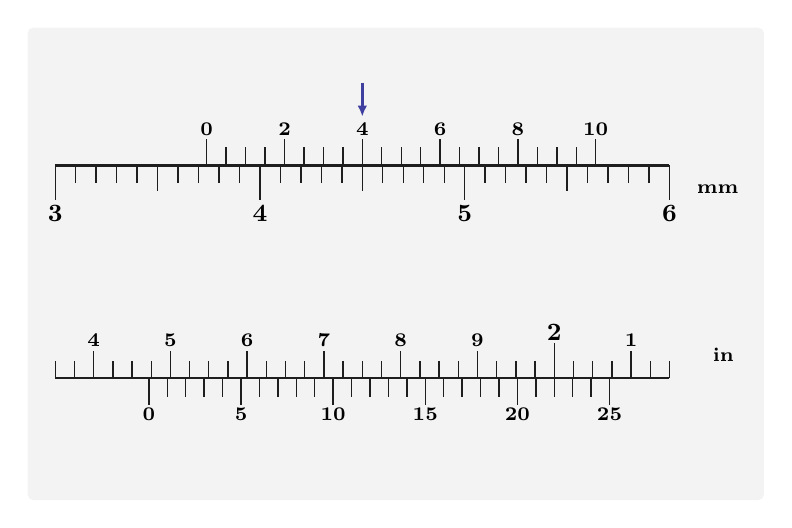
\begin{tikzpicture}[scale=1]
  \fill[figpanel,rounded corners=2pt] (-0.35,-1.55) rectangle (9,4.45);
  \begin{scope}[yshift=2.70cm]
  \draw[scb] (0,0) -- (7.8,0);
  \draw[sc] (0,0) -- (0,-0.44);
  \node[lab,below] at (0,-0.46) {3};
  \draw[sc] (0.26,0) -- (0.26,-0.22);
  \draw[sc] (0.52,0) -- (0.52,-0.22);
  \draw[sc] (0.78,0) -- (0.78,-0.22);
  \draw[sc] (1.04,0) -- (1.04,-0.22);
  \draw[sc] (1.3,0) -- (1.3,-0.32);
  \draw[sc] (1.56,0) -- (1.56,-0.22);
  \draw[sc] (1.82,0) -- (1.82,-0.22);
  \draw[sc] (2.08,0) -- (2.08,-0.22);
  \draw[sc] (2.34,0) -- (2.34,-0.22);
  \draw[sc] (2.6,0) -- (2.6,-0.44);
  \node[lab,below] at (2.6,-0.46) {4};
  \draw[sc] (2.86,0) -- (2.86,-0.22);
  \draw[sc] (3.12,0) -- (3.12,-0.22);
  \draw[sc] (3.38,0) -- (3.38,-0.22);
  \draw[sc] (3.64,0) -- (3.64,-0.22);
  \draw[sc] (3.9,0) -- (3.9,-0.32);
  \draw[sc] (4.16,0) -- (4.16,-0.22);
  \draw[sc] (4.42,0) -- (4.42,-0.22);
  \draw[sc] (4.68,0) -- (4.68,-0.22);
  \draw[sc] (4.94,0) -- (4.94,-0.22);
  \draw[sc] (5.2,0) -- (5.2,-0.44);
  \node[lab,below] at (5.2,-0.46) {5};
  \draw[sc] (5.46,0) -- (5.46,-0.22);
  \draw[sc] (5.72,0) -- (5.72,-0.22);
  \draw[sc] (5.98,0) -- (5.98,-0.22);
  \draw[sc] (6.24,0) -- (6.24,-0.22);
  \draw[sc] (6.5,0) -- (6.5,-0.32);
  \draw[sc] (6.76,0) -- (6.76,-0.22);
  \draw[sc] (7.02,0) -- (7.02,-0.22);
  \draw[sc] (7.28,0) -- (7.28,-0.22);
  \draw[sc] (7.54,0) -- (7.54,-0.22);
  \draw[sc] (7.8,0) -- (7.8,-0.44);
  \node[lab,below] at (7.8,-0.46) {6};
  \draw[sc] (1.924,0) -- (1.924,0.34);
  \node[labs,above] at (1.924,0.34) {0};
  \draw[sc] (2.171,0) -- (2.171,0.24);
  \draw[sc] (2.418,0) -- (2.418,0.24);
  \draw[sc] (2.665,0) -- (2.665,0.24);
  \draw[sc] (2.912,0) -- (2.912,0.34);
  \node[labs,above] at (2.912,0.34) {2};
  \draw[sc] (3.159,0) -- (3.159,0.24);
  \draw[sc] (3.406,0) -- (3.406,0.24);
  \draw[sc] (3.653,0) -- (3.653,0.24);
  \draw[sc] (3.9,0) -- (3.9,0.34);
  \node[labs,above] at (3.9,0.34) {4};
  \draw[sc] (4.147,0) -- (4.147,0.24);
  \draw[sc] (4.394,0) -- (4.394,0.24);
  \draw[sc] (4.641,0) -- (4.641,0.24);
  \draw[sc] (4.888,0) -- (4.888,0.34);
  \node[labs,above] at (4.888,0.34) {6};
  \draw[sc] (5.135,0) -- (5.135,0.24);
  \draw[sc] (5.382,0) -- (5.382,0.24);
  \draw[sc] (5.629,0) -- (5.629,0.24);
  \draw[sc] (5.876,0) -- (5.876,0.34);
  \node[labs,above] at (5.876,0.34) {8};
  \draw[sc] (6.123,0) -- (6.123,0.24);
  \draw[sc] (6.37,0) -- (6.37,0.24);
  \draw[sc] (6.617,0) -- (6.617,0.24);
  \draw[sc] (6.864,0) -- (6.864,0.34);
  \node[labs,above] at (6.864,0.34) {10};
  \draw[ptr] (3.9,1.05) -- (3.9,0.62);
  \node[labs,left] at (8.72,-0.30) {mm};
  \end{scope}
  \begin{scope}[yshift=0cm]
  \draw[scb] (0,0) -- (7.8,0);
  \draw[sc] (0,0) -- (0,0.22);
  \draw[sc] (0.2437,0) -- (0.2437,0.22);
  \draw[sc] (0.4875,0) -- (0.4875,0.34);
  \node[labs,above] at (0.4875,0.36) {4};
  \draw[sc] (0.7312,0) -- (0.7312,0.22);
  \draw[sc] (0.975,0) -- (0.975,0.22);
  \draw[sc] (1.2188,0) -- (1.2188,0.22);
  \draw[sc] (1.4625,0) -- (1.4625,0.34);
  \node[labs,above] at (1.4625,0.36) {5};
  \draw[sc] (1.7063,0) -- (1.7063,0.22);
  \draw[sc] (1.95,0) -- (1.95,0.22);
  \draw[sc] (2.1938,0) -- (2.1938,0.22);
  \draw[sc] (2.4375,0) -- (2.4375,0.34);
  \node[labs,above] at (2.4375,0.36) {6};
  \draw[sc] (2.6812,0) -- (2.6812,0.22);
  \draw[sc] (2.925,0) -- (2.925,0.22);
  \draw[sc] (3.1687,0) -- (3.1687,0.22);
  \draw[sc] (3.4125,0) -- (3.4125,0.34);
  \node[labs,above] at (3.4125,0.36) {7};
  \draw[sc] (3.6562,0) -- (3.6562,0.22);
  \draw[sc] (3.9,0) -- (3.9,0.22);
  \draw[sc] (4.1438,0) -- (4.1438,0.22);
  \draw[sc] (4.3875,0) -- (4.3875,0.34);
  \node[labs,above] at (4.3875,0.36) {8};
  \draw[sc] (4.6313,0) -- (4.6313,0.22);
  \draw[sc] (4.875,0) -- (4.875,0.22);
  \draw[sc] (5.1187,0) -- (5.1187,0.22);
  \draw[sc] (5.3625,0) -- (5.3625,0.34);
  \node[labs,above] at (5.3625,0.36) {9};
  \draw[sc] (5.6062,0) -- (5.6062,0.22);
  \draw[sc] (5.85,0) -- (5.85,0.22);
  \draw[sc] (6.0938,0) -- (6.0938,0.22);
  \draw[sc] (6.3375,0) -- (6.3375,0.44);
  \node[lab,above] at (6.3375,0.44) {2};
  \draw[sc] (6.5812,0) -- (6.5812,0.22);
  \draw[sc] (6.825,0) -- (6.825,0.22);
  \draw[sc] (7.0688,0) -- (7.0688,0.22);
  \draw[sc] (7.3125,0) -- (7.3125,0.34);
  \node[labs,above] at (7.3125,0.36) {1};
  \draw[sc] (7.5562,0) -- (7.5562,0.22);
  \draw[sc] (7.8,0) -- (7.8,0.22);
  \draw[sc] (1.1895,0) -- (1.1895,-0.34);
  \node[labs,below] at (1.1895,-0.34) {0};
  \draw[sc] (1.4235,0) -- (1.4235,-0.24);
  \draw[sc] (1.6575,0) -- (1.6575,-0.24);
  \draw[sc] (1.8915,0) -- (1.8915,-0.24);
  \draw[sc] (2.1255,0) -- (2.1255,-0.24);
  \draw[sc] (2.3595,0) -- (2.3595,-0.34);
  \node[labs,below] at (2.3595,-0.34) {5};
  \draw[sc] (2.5935,0) -- (2.5935,-0.24);
  \draw[sc] (2.8275,0) -- (2.8275,-0.24);
  \draw[sc] (3.0615,0) -- (3.0615,-0.24);
  \draw[sc] (3.2955,0) -- (3.2955,-0.24);
  \draw[sc] (3.5295,0) -- (3.5295,-0.34);
  \node[labs,below] at (3.5295,-0.34) {10};
  \draw[sc] (3.7635,0) -- (3.7635,-0.24);
  \draw[sc] (3.9975,0) -- (3.9975,-0.24);
  \draw[sc] (4.2315,0) -- (4.2315,-0.24);
  \draw[sc] (4.4655,0) -- (4.4655,-0.24);
  \draw[sc] (4.6995,0) -- (4.6995,-0.34);
  \node[labs,below] at (4.6995,-0.34) {15};
  \draw[sc] (4.9335,0) -- (4.9335,-0.24);
  \draw[sc] (5.1675,0) -- (5.1675,-0.24);
  \draw[sc] (5.4015,0) -- (5.4015,-0.24);
  \draw[sc] (5.6355,0) -- (5.6355,-0.24);
  \draw[sc] (5.8695,0) -- (5.8695,-0.34);
  \node[labs,below] at (5.8695,-0.34) {20};
  \draw[sc] (6.1035,0) -- (6.1035,-0.24);
  \draw[sc] (6.3375,0) -- (6.3375,-0.24);
  \draw[sc] (6.5715,0) -- (6.5715,-0.24);
  \draw[sc] (6.8055,0) -- (6.8055,-0.24);
  \draw[sc] (7.0395,0) -- (7.0395,-0.34);
  \node[labs,below] at (7.0395,-0.34) {25};
  \node[labs,left] at (8.66,0.30) {in};
  \end{scope}
\end{tikzpicture}
}

\newcommand{\figQBA}{%
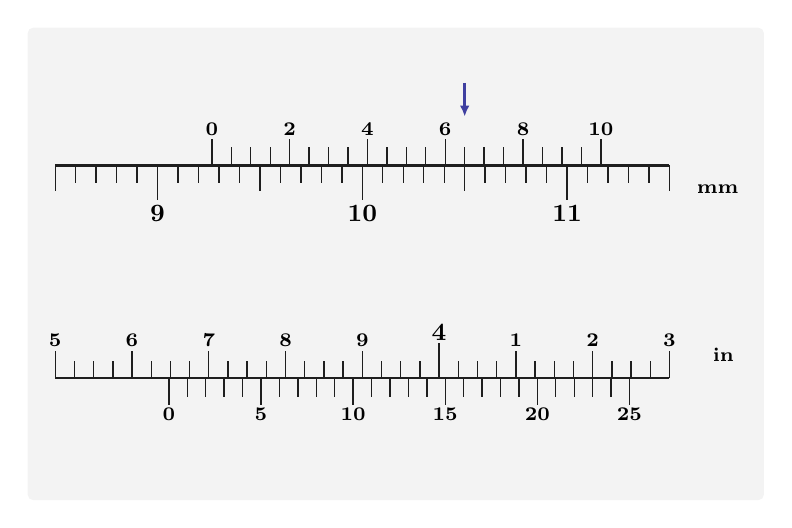
\begin{tikzpicture}[scale=1]
  \fill[figpanel,rounded corners=2pt] (-0.35,-1.55) rectangle (9,4.45);
  \begin{scope}[yshift=2.70cm]
  \draw[scb] (0,0) -- (7.8,0);
  \draw[sc] (0,0) -- (0,-0.32);
  \draw[sc] (0.26,0) -- (0.26,-0.22);
  \draw[sc] (0.52,0) -- (0.52,-0.22);
  \draw[sc] (0.78,0) -- (0.78,-0.22);
  \draw[sc] (1.04,0) -- (1.04,-0.22);
  \draw[sc] (1.3,0) -- (1.3,-0.44);
  \node[lab,below] at (1.3,-0.46) {9};
  \draw[sc] (1.56,0) -- (1.56,-0.22);
  \draw[sc] (1.82,0) -- (1.82,-0.22);
  \draw[sc] (2.08,0) -- (2.08,-0.22);
  \draw[sc] (2.34,0) -- (2.34,-0.22);
  \draw[sc] (2.6,0) -- (2.6,-0.32);
  \draw[sc] (2.86,0) -- (2.86,-0.22);
  \draw[sc] (3.12,0) -- (3.12,-0.22);
  \draw[sc] (3.38,0) -- (3.38,-0.22);
  \draw[sc] (3.64,0) -- (3.64,-0.22);
  \draw[sc] (3.9,0) -- (3.9,-0.44);
  \node[lab,below] at (3.9,-0.46) {10};
  \draw[sc] (4.16,0) -- (4.16,-0.22);
  \draw[sc] (4.42,0) -- (4.42,-0.22);
  \draw[sc] (4.68,0) -- (4.68,-0.22);
  \draw[sc] (4.94,0) -- (4.94,-0.22);
  \draw[sc] (5.2,0) -- (5.2,-0.32);
  \draw[sc] (5.46,0) -- (5.46,-0.22);
  \draw[sc] (5.72,0) -- (5.72,-0.22);
  \draw[sc] (5.98,0) -- (5.98,-0.22);
  \draw[sc] (6.24,0) -- (6.24,-0.22);
  \draw[sc] (6.5,0) -- (6.5,-0.44);
  \node[lab,below] at (6.5,-0.46) {11};
  \draw[sc] (6.76,0) -- (6.76,-0.22);
  \draw[sc] (7.02,0) -- (7.02,-0.22);
  \draw[sc] (7.28,0) -- (7.28,-0.22);
  \draw[sc] (7.54,0) -- (7.54,-0.22);
  \draw[sc] (7.8,0) -- (7.8,-0.32);
  \draw[sc] (1.989,0) -- (1.989,0.34);
  \node[labs,above] at (1.989,0.34) {0};
  \draw[sc] (2.236,0) -- (2.236,0.24);
  \draw[sc] (2.483,0) -- (2.483,0.24);
  \draw[sc] (2.73,0) -- (2.73,0.24);
  \draw[sc] (2.977,0) -- (2.977,0.34);
  \node[labs,above] at (2.977,0.34) {2};
  \draw[sc] (3.224,0) -- (3.224,0.24);
  \draw[sc] (3.471,0) -- (3.471,0.24);
  \draw[sc] (3.718,0) -- (3.718,0.24);
  \draw[sc] (3.965,0) -- (3.965,0.34);
  \node[labs,above] at (3.965,0.34) {4};
  \draw[sc] (4.212,0) -- (4.212,0.24);
  \draw[sc] (4.459,0) -- (4.459,0.24);
  \draw[sc] (4.706,0) -- (4.706,0.24);
  \draw[sc] (4.953,0) -- (4.953,0.34);
  \node[labs,above] at (4.953,0.34) {6};
  \draw[sc] (5.2,0) -- (5.2,0.24);
  \draw[sc] (5.447,0) -- (5.447,0.24);
  \draw[sc] (5.694,0) -- (5.694,0.24);
  \draw[sc] (5.941,0) -- (5.941,0.34);
  \node[labs,above] at (5.941,0.34) {8};
  \draw[sc] (6.188,0) -- (6.188,0.24);
  \draw[sc] (6.435,0) -- (6.435,0.24);
  \draw[sc] (6.682,0) -- (6.682,0.24);
  \draw[sc] (6.929,0) -- (6.929,0.34);
  \node[labs,above] at (6.929,0.34) {10};
  \draw[ptr] (5.2,1.05) -- (5.2,0.62);
  \node[labs,left] at (8.72,-0.30) {mm};
  \end{scope}
  \begin{scope}[yshift=0cm]
  \draw[scb] (0,0) -- (7.8,0);
  \draw[sc] (0,0) -- (0,0.34);
  \node[labs,above] at (0,0.36) {5};
  \draw[sc] (0.2438,0) -- (0.2438,0.22);
  \draw[sc] (0.4875,0) -- (0.4875,0.22);
  \draw[sc] (0.7313,0) -- (0.7313,0.22);
  \draw[sc] (0.975,0) -- (0.975,0.34);
  \node[labs,above] at (0.975,0.36) {6};
  \draw[sc] (1.2188,0) -- (1.2188,0.22);
  \draw[sc] (1.4625,0) -- (1.4625,0.22);
  \draw[sc] (1.7063,0) -- (1.7063,0.22);
  \draw[sc] (1.95,0) -- (1.95,0.34);
  \node[labs,above] at (1.95,0.36) {7};
  \draw[sc] (2.1938,0) -- (2.1938,0.22);
  \draw[sc] (2.4375,0) -- (2.4375,0.22);
  \draw[sc] (2.6813,0) -- (2.6813,0.22);
  \draw[sc] (2.925,0) -- (2.925,0.34);
  \node[labs,above] at (2.925,0.36) {8};
  \draw[sc] (3.1688,0) -- (3.1688,0.22);
  \draw[sc] (3.4125,0) -- (3.4125,0.22);
  \draw[sc] (3.6562,0) -- (3.6562,0.22);
  \draw[sc] (3.9,0) -- (3.9,0.34);
  \node[labs,above] at (3.9,0.36) {9};
  \draw[sc] (4.1438,0) -- (4.1438,0.22);
  \draw[sc] (4.3875,0) -- (4.3875,0.22);
  \draw[sc] (4.6313,0) -- (4.6313,0.22);
  \draw[sc] (4.875,0) -- (4.875,0.44);
  \node[lab,above] at (4.875,0.44) {4};
  \draw[sc] (5.1188,0) -- (5.1188,0.22);
  \draw[sc] (5.3625,0) -- (5.3625,0.22);
  \draw[sc] (5.6063,0) -- (5.6063,0.22);
  \draw[sc] (5.85,0) -- (5.85,0.34);
  \node[labs,above] at (5.85,0.36) {1};
  \draw[sc] (6.0938,0) -- (6.0938,0.22);
  \draw[sc] (6.3375,0) -- (6.3375,0.22);
  \draw[sc] (6.5812,0) -- (6.5812,0.22);
  \draw[sc] (6.825,0) -- (6.825,0.34);
  \node[labs,above] at (6.825,0.36) {2};
  \draw[sc] (7.0688,0) -- (7.0688,0.22);
  \draw[sc] (7.3125,0) -- (7.3125,0.22);
  \draw[sc] (7.5563,0) -- (7.5563,0.22);
  \draw[sc] (7.8,0) -- (7.8,0.34);
  \node[labs,above] at (7.8,0.36) {3};
  \draw[sc] (1.443,0) -- (1.443,-0.34);
  \node[labs,below] at (1.443,-0.34) {0};
  \draw[sc] (1.677,0) -- (1.677,-0.24);
  \draw[sc] (1.911,0) -- (1.911,-0.24);
  \draw[sc] (2.145,0) -- (2.145,-0.24);
  \draw[sc] (2.379,0) -- (2.379,-0.24);
  \draw[sc] (2.613,0) -- (2.613,-0.34);
  \node[labs,below] at (2.613,-0.34) {5};
  \draw[sc] (2.847,0) -- (2.847,-0.24);
  \draw[sc] (3.081,0) -- (3.081,-0.24);
  \draw[sc] (3.315,0) -- (3.315,-0.24);
  \draw[sc] (3.549,0) -- (3.549,-0.24);
  \draw[sc] (3.783,0) -- (3.783,-0.34);
  \node[labs,below] at (3.783,-0.34) {10};
  \draw[sc] (4.017,0) -- (4.017,-0.24);
  \draw[sc] (4.251,0) -- (4.251,-0.24);
  \draw[sc] (4.485,0) -- (4.485,-0.24);
  \draw[sc] (4.719,0) -- (4.719,-0.24);
  \draw[sc] (4.953,0) -- (4.953,-0.34);
  \node[labs,below] at (4.953,-0.34) {15};
  \draw[sc] (5.187,0) -- (5.187,-0.24);
  \draw[sc] (5.421,0) -- (5.421,-0.24);
  \draw[sc] (5.655,0) -- (5.655,-0.24);
  \draw[sc] (5.889,0) -- (5.889,-0.24);
  \draw[sc] (6.123,0) -- (6.123,-0.34);
  \node[labs,below] at (6.123,-0.34) {20};
  \draw[sc] (6.357,0) -- (6.357,-0.24);
  \draw[sc] (6.591,0) -- (6.591,-0.24);
  \draw[sc] (6.825,0) -- (6.825,-0.24);
  \draw[sc] (7.059,0) -- (7.059,-0.24);
  \draw[sc] (7.293,0) -- (7.293,-0.34);
  \node[labs,below] at (7.293,-0.34) {25};
  \node[labs,left] at (8.66,0.30) {in};
  \end{scope}
\end{tikzpicture}
}

\newcommand{\figQBB}{%
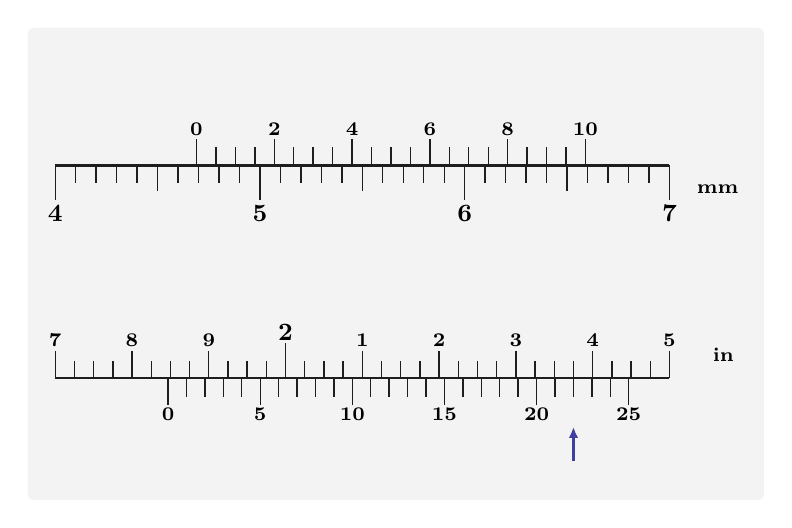
\begin{tikzpicture}[scale=1]
  \fill[figpanel,rounded corners=2pt] (-0.35,-1.55) rectangle (9,4.45);
  \begin{scope}[yshift=2.70cm]
  \draw[scb] (0,0) -- (7.8,0);
  \draw[sc] (0,0) -- (0,-0.44);
  \node[lab,below] at (0,-0.46) {4};
  \draw[sc] (0.26,0) -- (0.26,-0.22);
  \draw[sc] (0.52,0) -- (0.52,-0.22);
  \draw[sc] (0.78,0) -- (0.78,-0.22);
  \draw[sc] (1.04,0) -- (1.04,-0.22);
  \draw[sc] (1.3,0) -- (1.3,-0.32);
  \draw[sc] (1.56,0) -- (1.56,-0.22);
  \draw[sc] (1.82,0) -- (1.82,-0.22);
  \draw[sc] (2.08,0) -- (2.08,-0.22);
  \draw[sc] (2.34,0) -- (2.34,-0.22);
  \draw[sc] (2.6,0) -- (2.6,-0.44);
  \node[lab,below] at (2.6,-0.46) {5};
  \draw[sc] (2.86,0) -- (2.86,-0.22);
  \draw[sc] (3.12,0) -- (3.12,-0.22);
  \draw[sc] (3.38,0) -- (3.38,-0.22);
  \draw[sc] (3.64,0) -- (3.64,-0.22);
  \draw[sc] (3.9,0) -- (3.9,-0.32);
  \draw[sc] (4.16,0) -- (4.16,-0.22);
  \draw[sc] (4.42,0) -- (4.42,-0.22);
  \draw[sc] (4.68,0) -- (4.68,-0.22);
  \draw[sc] (4.94,0) -- (4.94,-0.22);
  \draw[sc] (5.2,0) -- (5.2,-0.44);
  \node[lab,below] at (5.2,-0.46) {6};
  \draw[sc] (5.46,0) -- (5.46,-0.22);
  \draw[sc] (5.72,0) -- (5.72,-0.22);
  \draw[sc] (5.98,0) -- (5.98,-0.22);
  \draw[sc] (6.24,0) -- (6.24,-0.22);
  \draw[sc] (6.5,0) -- (6.5,-0.32);
  \draw[sc] (6.76,0) -- (6.76,-0.22);
  \draw[sc] (7.02,0) -- (7.02,-0.22);
  \draw[sc] (7.28,0) -- (7.28,-0.22);
  \draw[sc] (7.54,0) -- (7.54,-0.22);
  \draw[sc] (7.8,0) -- (7.8,-0.44);
  \node[lab,below] at (7.8,-0.46) {7};
  \draw[sc] (1.794,0) -- (1.794,0.34);
  \node[labs,above] at (1.794,0.34) {0};
  \draw[sc] (2.041,0) -- (2.041,0.24);
  \draw[sc] (2.288,0) -- (2.288,0.24);
  \draw[sc] (2.535,0) -- (2.535,0.24);
  \draw[sc] (2.782,0) -- (2.782,0.34);
  \node[labs,above] at (2.782,0.34) {2};
  \draw[sc] (3.029,0) -- (3.029,0.24);
  \draw[sc] (3.276,0) -- (3.276,0.24);
  \draw[sc] (3.523,0) -- (3.523,0.24);
  \draw[sc] (3.77,0) -- (3.77,0.34);
  \node[labs,above] at (3.77,0.34) {4};
  \draw[sc] (4.017,0) -- (4.017,0.24);
  \draw[sc] (4.264,0) -- (4.264,0.24);
  \draw[sc] (4.511,0) -- (4.511,0.24);
  \draw[sc] (4.758,0) -- (4.758,0.34);
  \node[labs,above] at (4.758,0.34) {6};
  \draw[sc] (5.005,0) -- (5.005,0.24);
  \draw[sc] (5.252,0) -- (5.252,0.24);
  \draw[sc] (5.499,0) -- (5.499,0.24);
  \draw[sc] (5.746,0) -- (5.746,0.34);
  \node[labs,above] at (5.746,0.34) {8};
  \draw[sc] (5.993,0) -- (5.993,0.24);
  \draw[sc] (6.24,0) -- (6.24,0.24);
  \draw[sc] (6.487,0) -- (6.487,0.24);
  \draw[sc] (6.734,0) -- (6.734,0.34);
  \node[labs,above] at (6.734,0.34) {10};
  \node[labs,left] at (8.72,-0.30) {mm};
  \end{scope}
  \begin{scope}[yshift=0cm]
  \draw[scb] (0,0) -- (7.8,0);
  \draw[sc] (0,0) -- (0,0.34);
  \node[labs,above] at (0,0.36) {7};
  \draw[sc] (0.2438,0) -- (0.2438,0.22);
  \draw[sc] (0.4875,0) -- (0.4875,0.22);
  \draw[sc] (0.7313,0) -- (0.7313,0.22);
  \draw[sc] (0.975,0) -- (0.975,0.34);
  \node[labs,above] at (0.975,0.36) {8};
  \draw[sc] (1.2188,0) -- (1.2188,0.22);
  \draw[sc] (1.4625,0) -- (1.4625,0.22);
  \draw[sc] (1.7063,0) -- (1.7063,0.22);
  \draw[sc] (1.95,0) -- (1.95,0.34);
  \node[labs,above] at (1.95,0.36) {9};
  \draw[sc] (2.1938,0) -- (2.1938,0.22);
  \draw[sc] (2.4375,0) -- (2.4375,0.22);
  \draw[sc] (2.6813,0) -- (2.6813,0.22);
  \draw[sc] (2.925,0) -- (2.925,0.44);
  \node[lab,above] at (2.925,0.44) {2};
  \draw[sc] (3.1687,0) -- (3.1687,0.22);
  \draw[sc] (3.4125,0) -- (3.4125,0.22);
  \draw[sc] (3.6563,0) -- (3.6563,0.22);
  \draw[sc] (3.9,0) -- (3.9,0.34);
  \node[labs,above] at (3.9,0.36) {1};
  \draw[sc] (4.1438,0) -- (4.1438,0.22);
  \draw[sc] (4.3875,0) -- (4.3875,0.22);
  \draw[sc] (4.6313,0) -- (4.6313,0.22);
  \draw[sc] (4.875,0) -- (4.875,0.34);
  \node[labs,above] at (4.875,0.36) {2};
  \draw[sc] (5.1188,0) -- (5.1188,0.22);
  \draw[sc] (5.3625,0) -- (5.3625,0.22);
  \draw[sc] (5.6062,0) -- (5.6062,0.22);
  \draw[sc] (5.85,0) -- (5.85,0.34);
  \node[labs,above] at (5.85,0.36) {3};
  \draw[sc] (6.0938,0) -- (6.0938,0.22);
  \draw[sc] (6.3375,0) -- (6.3375,0.22);
  \draw[sc] (6.5813,0) -- (6.5813,0.22);
  \draw[sc] (6.825,0) -- (6.825,0.34);
  \node[labs,above] at (6.825,0.36) {4};
  \draw[sc] (7.0688,0) -- (7.0688,0.22);
  \draw[sc] (7.3125,0) -- (7.3125,0.22);
  \draw[sc] (7.5563,0) -- (7.5563,0.22);
  \draw[sc] (7.8,0) -- (7.8,0.34);
  \node[labs,above] at (7.8,0.36) {5};
  \draw[sc] (1.4333,0) -- (1.4333,-0.34);
  \node[labs,below] at (1.4333,-0.34) {0};
  \draw[sc] (1.6673,0) -- (1.6673,-0.24);
  \draw[sc] (1.9013,0) -- (1.9013,-0.24);
  \draw[sc] (2.1353,0) -- (2.1353,-0.24);
  \draw[sc] (2.3693,0) -- (2.3693,-0.24);
  \draw[sc] (2.6033,0) -- (2.6033,-0.34);
  \node[labs,below] at (2.6033,-0.34) {5};
  \draw[sc] (2.8373,0) -- (2.8373,-0.24);
  \draw[sc] (3.0713,0) -- (3.0713,-0.24);
  \draw[sc] (3.3053,0) -- (3.3053,-0.24);
  \draw[sc] (3.5393,0) -- (3.5393,-0.24);
  \draw[sc] (3.7732,0) -- (3.7732,-0.34);
  \node[labs,below] at (3.7732,-0.34) {10};
  \draw[sc] (4.0072,0) -- (4.0072,-0.24);
  \draw[sc] (4.2412,0) -- (4.2412,-0.24);
  \draw[sc] (4.4752,0) -- (4.4752,-0.24);
  \draw[sc] (4.7092,0) -- (4.7092,-0.24);
  \draw[sc] (4.9432,0) -- (4.9432,-0.34);
  \node[labs,below] at (4.9432,-0.34) {15};
  \draw[sc] (5.1772,0) -- (5.1772,-0.24);
  \draw[sc] (5.4112,0) -- (5.4112,-0.24);
  \draw[sc] (5.6452,0) -- (5.6452,-0.24);
  \draw[sc] (5.8792,0) -- (5.8792,-0.24);
  \draw[sc] (6.1132,0) -- (6.1132,-0.34);
  \node[labs,below] at (6.1132,-0.34) {20};
  \draw[sc] (6.3472,0) -- (6.3472,-0.24);
  \draw[sc] (6.5813,0) -- (6.5813,-0.24);
  \draw[sc] (6.8153,0) -- (6.8153,-0.24);
  \draw[sc] (7.0493,0) -- (7.0493,-0.24);
  \draw[sc] (7.2833,0) -- (7.2833,-0.34);
  \node[labs,below] at (7.2833,-0.34) {25};
  \draw[ptr] (6.5813,-1.05) -- (6.5813,-0.62);
  \node[labs,left] at (8.66,0.30) {in};
  \end{scope}
\end{tikzpicture}
}

\newcommand{\figQBC}{%
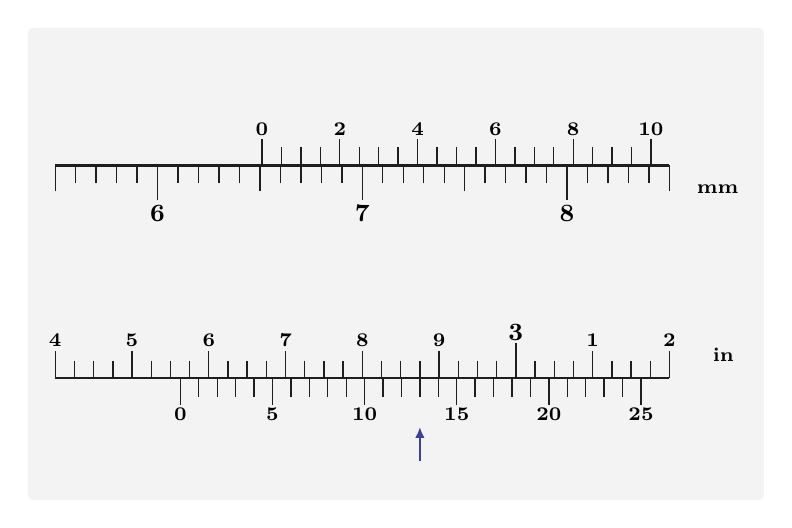
\begin{tikzpicture}[scale=1]
  \fill[figpanel,rounded corners=2pt] (-0.35,-1.55) rectangle (9,4.45);
  \begin{scope}[yshift=2.70cm]
  \draw[scb] (0,0) -- (7.8,0);
  \draw[sc] (0,0) -- (0,-0.32);
  \draw[sc] (0.26,0) -- (0.26,-0.22);
  \draw[sc] (0.52,0) -- (0.52,-0.22);
  \draw[sc] (0.78,0) -- (0.78,-0.22);
  \draw[sc] (1.04,0) -- (1.04,-0.22);
  \draw[sc] (1.3,0) -- (1.3,-0.44);
  \node[lab,below] at (1.3,-0.46) {6};
  \draw[sc] (1.56,0) -- (1.56,-0.22);
  \draw[sc] (1.82,0) -- (1.82,-0.22);
  \draw[sc] (2.08,0) -- (2.08,-0.22);
  \draw[sc] (2.34,0) -- (2.34,-0.22);
  \draw[sc] (2.6,0) -- (2.6,-0.32);
  \draw[sc] (2.86,0) -- (2.86,-0.22);
  \draw[sc] (3.12,0) -- (3.12,-0.22);
  \draw[sc] (3.38,0) -- (3.38,-0.22);
  \draw[sc] (3.64,0) -- (3.64,-0.22);
  \draw[sc] (3.9,0) -- (3.9,-0.44);
  \node[lab,below] at (3.9,-0.46) {7};
  \draw[sc] (4.16,0) -- (4.16,-0.22);
  \draw[sc] (4.42,0) -- (4.42,-0.22);
  \draw[sc] (4.68,0) -- (4.68,-0.22);
  \draw[sc] (4.94,0) -- (4.94,-0.22);
  \draw[sc] (5.2,0) -- (5.2,-0.32);
  \draw[sc] (5.46,0) -- (5.46,-0.22);
  \draw[sc] (5.72,0) -- (5.72,-0.22);
  \draw[sc] (5.98,0) -- (5.98,-0.22);
  \draw[sc] (6.24,0) -- (6.24,-0.22);
  \draw[sc] (6.5,0) -- (6.5,-0.44);
  \node[lab,below] at (6.5,-0.46) {8};
  \draw[sc] (6.76,0) -- (6.76,-0.22);
  \draw[sc] (7.02,0) -- (7.02,-0.22);
  \draw[sc] (7.28,0) -- (7.28,-0.22);
  \draw[sc] (7.54,0) -- (7.54,-0.22);
  \draw[sc] (7.8,0) -- (7.8,-0.32);
  \draw[sc] (2.626,0) -- (2.626,0.34);
  \node[labs,above] at (2.626,0.34) {0};
  \draw[sc] (2.873,0) -- (2.873,0.24);
  \draw[sc] (3.12,0) -- (3.12,0.24);
  \draw[sc] (3.367,0) -- (3.367,0.24);
  \draw[sc] (3.614,0) -- (3.614,0.34);
  \node[labs,above] at (3.614,0.34) {2};
  \draw[sc] (3.861,0) -- (3.861,0.24);
  \draw[sc] (4.108,0) -- (4.108,0.24);
  \draw[sc] (4.355,0) -- (4.355,0.24);
  \draw[sc] (4.602,0) -- (4.602,0.34);
  \node[labs,above] at (4.602,0.34) {4};
  \draw[sc] (4.849,0) -- (4.849,0.24);
  \draw[sc] (5.096,0) -- (5.096,0.24);
  \draw[sc] (5.343,0) -- (5.343,0.24);
  \draw[sc] (5.59,0) -- (5.59,0.34);
  \node[labs,above] at (5.59,0.34) {6};
  \draw[sc] (5.837,0) -- (5.837,0.24);
  \draw[sc] (6.084,0) -- (6.084,0.24);
  \draw[sc] (6.331,0) -- (6.331,0.24);
  \draw[sc] (6.578,0) -- (6.578,0.34);
  \node[labs,above] at (6.578,0.34) {8};
  \draw[sc] (6.825,0) -- (6.825,0.24);
  \draw[sc] (7.072,0) -- (7.072,0.24);
  \draw[sc] (7.319,0) -- (7.319,0.24);
  \draw[sc] (7.566,0) -- (7.566,0.34);
  \node[labs,above] at (7.566,0.34) {10};
  \node[labs,left] at (8.72,-0.30) {mm};
  \end{scope}
  \begin{scope}[yshift=0cm]
  \draw[scb] (0,0) -- (7.8,0);
  \draw[sc] (0,0) -- (0,0.34);
  \node[labs,above] at (0,0.36) {4};
  \draw[sc] (0.2438,0) -- (0.2438,0.22);
  \draw[sc] (0.4875,0) -- (0.4875,0.22);
  \draw[sc] (0.7313,0) -- (0.7313,0.22);
  \draw[sc] (0.975,0) -- (0.975,0.34);
  \node[labs,above] at (0.975,0.36) {5};
  \draw[sc] (1.2188,0) -- (1.2188,0.22);
  \draw[sc] (1.4625,0) -- (1.4625,0.22);
  \draw[sc] (1.7063,0) -- (1.7063,0.22);
  \draw[sc] (1.95,0) -- (1.95,0.34);
  \node[labs,above] at (1.95,0.36) {6};
  \draw[sc] (2.1938,0) -- (2.1938,0.22);
  \draw[sc] (2.4375,0) -- (2.4375,0.22);
  \draw[sc] (2.6813,0) -- (2.6813,0.22);
  \draw[sc] (2.925,0) -- (2.925,0.34);
  \node[labs,above] at (2.925,0.36) {7};
  \draw[sc] (3.1688,0) -- (3.1688,0.22);
  \draw[sc] (3.4125,0) -- (3.4125,0.22);
  \draw[sc] (3.6563,0) -- (3.6563,0.22);
  \draw[sc] (3.9,0) -- (3.9,0.34);
  \node[labs,above] at (3.9,0.36) {8};
  \draw[sc] (4.1438,0) -- (4.1438,0.22);
  \draw[sc] (4.3875,0) -- (4.3875,0.22);
  \draw[sc] (4.6313,0) -- (4.6313,0.22);
  \draw[sc] (4.875,0) -- (4.875,0.34);
  \node[labs,above] at (4.875,0.36) {9};
  \draw[sc] (5.1188,0) -- (5.1188,0.22);
  \draw[sc] (5.3625,0) -- (5.3625,0.22);
  \draw[sc] (5.6063,0) -- (5.6063,0.22);
  \draw[sc] (5.85,0) -- (5.85,0.44);
  \node[lab,above] at (5.85,0.44) {3};
  \draw[sc] (6.0938,0) -- (6.0938,0.22);
  \draw[sc] (6.3375,0) -- (6.3375,0.22);
  \draw[sc] (6.5813,0) -- (6.5813,0.22);
  \draw[sc] (6.825,0) -- (6.825,0.34);
  \node[labs,above] at (6.825,0.36) {1};
  \draw[sc] (7.0688,0) -- (7.0688,0.22);
  \draw[sc] (7.3125,0) -- (7.3125,0.22);
  \draw[sc] (7.5563,0) -- (7.5563,0.22);
  \draw[sc] (7.8,0) -- (7.8,0.34);
  \node[labs,above] at (7.8,0.36) {2};
  \draw[sc] (1.5893,0) -- (1.5893,-0.34);
  \node[labs,below] at (1.5893,-0.34) {0};
  \draw[sc] (1.8233,0) -- (1.8233,-0.24);
  \draw[sc] (2.0573,0) -- (2.0573,-0.24);
  \draw[sc] (2.2913,0) -- (2.2913,-0.24);
  \draw[sc] (2.5253,0) -- (2.5253,-0.24);
  \draw[sc] (2.7593,0) -- (2.7593,-0.34);
  \node[labs,below] at (2.7593,-0.34) {5};
  \draw[sc] (2.9933,0) -- (2.9933,-0.24);
  \draw[sc] (3.2273,0) -- (3.2273,-0.24);
  \draw[sc] (3.4613,0) -- (3.4613,-0.24);
  \draw[sc] (3.6953,0) -- (3.6953,-0.24);
  \draw[sc] (3.9293,0) -- (3.9293,-0.34);
  \node[labs,below] at (3.9293,-0.34) {10};
  \draw[sc] (4.1633,0) -- (4.1633,-0.24);
  \draw[sc] (4.3973,0) -- (4.3973,-0.24);
  \draw[sc] (4.6313,0) -- (4.6313,-0.24);
  \draw[sc] (4.8653,0) -- (4.8653,-0.24);
  \draw[sc] (5.0993,0) -- (5.0993,-0.34);
  \node[labs,below] at (5.0993,-0.34) {15};
  \draw[sc] (5.3333,0) -- (5.3333,-0.24);
  \draw[sc] (5.5673,0) -- (5.5673,-0.24);
  \draw[sc] (5.8013,0) -- (5.8013,-0.24);
  \draw[sc] (6.0353,0) -- (6.0353,-0.24);
  \draw[sc] (6.2693,0) -- (6.2693,-0.34);
  \node[labs,below] at (6.2693,-0.34) {20};
  \draw[sc] (6.5033,0) -- (6.5033,-0.24);
  \draw[sc] (6.7373,0) -- (6.7373,-0.24);
  \draw[sc] (6.9713,0) -- (6.9713,-0.24);
  \draw[sc] (7.2053,0) -- (7.2053,-0.24);
  \draw[sc] (7.4393,0) -- (7.4393,-0.34);
  \node[labs,below] at (7.4393,-0.34) {25};
  \draw[ptr] (4.6313,-1.05) -- (4.6313,-0.62);
  \node[labs,left] at (8.66,0.30) {in};
  \end{scope}
\end{tikzpicture}
}

\newcommand{\figQBF}{%
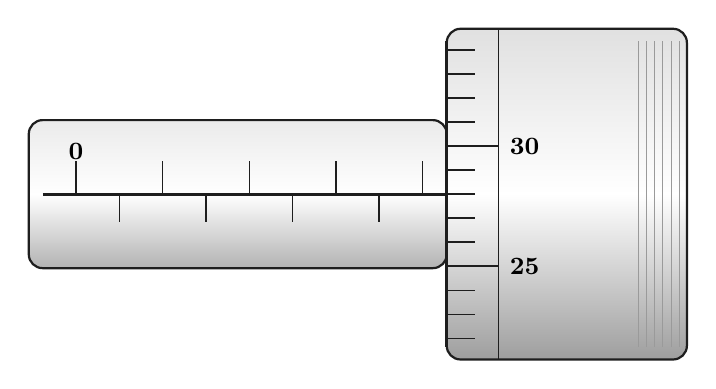
\begin{tikzpicture}[scale=1]
  \shade[rounded corners=5pt,top color=black!8,bottom color=black!30,middle color=white] (0,-0.94) rectangle (5.308,0.94);
  \draw[scb,rounded corners=5pt] (0,-0.94) rectangle (5.308,0.94);
  \draw[draw=figline,line width=1.1pt] (0.18,0) -- (5.308,0);
  \draw[sc] (0.6,0) -- (0.6,0.42);
  \node[lab,above] at (0.6,0.40) {0};
  \draw[sc] (1.15,0) -- (1.15,-0.36);
  \draw[sc] (1.7,0) -- (1.7,0.42);
  \draw[sc] (2.25,0) -- (2.25,-0.36);
  \draw[sc] (2.8,0) -- (2.8,0.42);
  \draw[sc] (3.35,0) -- (3.35,-0.36);
  \draw[sc] (3.9,0) -- (3.9,0.42);
  \draw[sc] (4.45,0) -- (4.45,-0.36);
  \draw[sc] (5,0) -- (5,0.42);
  \shade[rounded corners=5pt,top color=black!12,bottom color=black!38,middle color=white] (5.308,-2.1) rectangle (8.358,2.1);
  \draw[scb,rounded corners=5pt] (5.308,-2.1) rectangle (8.358,2.1);
  \draw[draw=figline,line width=1.0pt] (5.308,-1.94) -- (5.308,1.94);
  \draw[sc] (5.968,-2.1) -- (5.968,2.1);
  \draw[draw=figline!45,line width=0.4pt] (7.738,-1.94) -- (7.738,1.94);
  \draw[draw=figline!45,line width=0.4pt] (7.843,-1.94) -- (7.843,1.94);
  \draw[draw=figline!45,line width=0.4pt] (7.948,-1.94) -- (7.948,1.94);
  \draw[draw=figline!45,line width=0.4pt] (8.053,-1.94) -- (8.053,1.94);
  \draw[draw=figline!45,line width=0.4pt] (8.158,-1.94) -- (8.158,1.94);
  \draw[draw=figline!45,line width=0.4pt] (8.263,-1.94) -- (8.263,1.94);
  \draw[draw=figline,line width=0.5pt] (5.308,-1.83) -- (5.671,-1.83);
  \draw[draw=figline,line width=0.5pt] (5.308,-1.525) -- (5.671,-1.525);
  \draw[draw=figline,line width=0.5pt] (5.308,-1.22) -- (5.671,-1.22);
  \draw[draw=figline,line width=0.9pt] (5.308,-0.915) -- (5.968,-0.915);
  \node[lab,right] at (6.068,-0.915) {25};
  \draw[draw=figline,line width=0.5pt] (5.308,-0.61) -- (5.671,-0.61);
  \draw[draw=figline,line width=0.5pt] (5.308,-0.305) -- (5.671,-0.305);
  \draw[draw=figline,line width=0.5pt] (5.308,0) -- (5.671,0);
  \draw[draw=figline,line width=0.5pt] (5.308,0.305) -- (5.671,0.305);
  \draw[draw=figline,line width=0.9pt] (5.308,0.61) -- (5.968,0.61);
  \node[lab,right] at (6.068,0.61) {30};
  \draw[draw=figline,line width=0.5pt] (5.308,0.915) -- (5.671,0.915);
  \draw[draw=figline,line width=0.5pt] (5.308,1.22) -- (5.671,1.22);
  \draw[draw=figline,line width=0.5pt] (5.308,1.525) -- (5.671,1.525);
  \draw[draw=figline,line width=0.5pt] (5.308,1.83) -- (5.671,1.83);
\end{tikzpicture}
}

\newcommand{\figQBG}{%
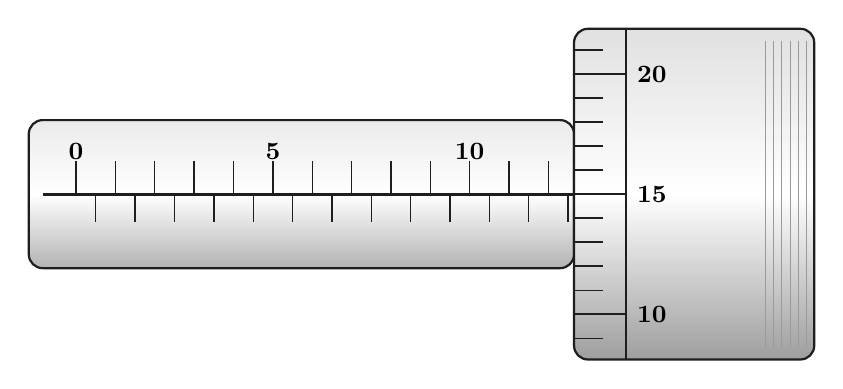
\begin{tikzpicture}[scale=1]
  \shade[rounded corners=5pt,top color=black!8,bottom color=black!30,middle color=white] (0,-0.94) rectangle (6.925,0.94);
  \draw[scb,rounded corners=5pt] (0,-0.94) rectangle (6.925,0.94);
  \draw[draw=figline,line width=1.1pt] (0.18,0) -- (6.925,0);
  \draw[sc] (0.6,0) -- (0.6,0.42);
  \node[lab,above] at (0.6,0.40) {0};
  \draw[sc] (0.85,0) -- (0.85,-0.36);
  \draw[sc] (1.1,0) -- (1.1,0.42);
  \draw[sc] (1.35,0) -- (1.35,-0.36);
  \draw[sc] (1.6,0) -- (1.6,0.42);
  \draw[sc] (1.85,0) -- (1.85,-0.36);
  \draw[sc] (2.1,0) -- (2.1,0.42);
  \draw[sc] (2.35,0) -- (2.35,-0.36);
  \draw[sc] (2.6,0) -- (2.6,0.42);
  \draw[sc] (2.85,0) -- (2.85,-0.36);
  \draw[sc] (3.1,0) -- (3.1,0.42);
  \node[lab,above] at (3.1,0.40) {5};
  \draw[sc] (3.35,0) -- (3.35,-0.36);
  \draw[sc] (3.6,0) -- (3.6,0.42);
  \draw[sc] (3.85,0) -- (3.85,-0.36);
  \draw[sc] (4.1,0) -- (4.1,0.42);
  \draw[sc] (4.35,0) -- (4.35,-0.36);
  \draw[sc] (4.6,0) -- (4.6,0.42);
  \draw[sc] (4.85,0) -- (4.85,-0.36);
  \draw[sc] (5.1,0) -- (5.1,0.42);
  \draw[sc] (5.35,0) -- (5.35,-0.36);
  \draw[sc] (5.6,0) -- (5.6,0.42);
  \node[lab,above] at (5.6,0.40) {10};
  \draw[sc] (5.85,0) -- (5.85,-0.36);
  \draw[sc] (6.1,0) -- (6.1,0.42);
  \draw[sc] (6.35,0) -- (6.35,-0.36);
  \draw[sc] (6.6,0) -- (6.6,0.42);
  \draw[sc] (6.85,0) -- (6.85,-0.36);
  \shade[rounded corners=5pt,top color=black!12,bottom color=black!38,middle color=white] (6.925,-2.1) rectangle (9.975,2.1);
  \draw[scb,rounded corners=5pt] (6.925,-2.1) rectangle (9.975,2.1);
  \draw[draw=figline,line width=1.0pt] (6.925,-1.94) -- (6.925,1.94);
  \draw[sc] (7.585,-2.1) -- (7.585,2.1);
  \draw[draw=figline!45,line width=0.4pt] (9.355,-1.94) -- (9.355,1.94);
  \draw[draw=figline!45,line width=0.4pt] (9.46,-1.94) -- (9.46,1.94);
  \draw[draw=figline!45,line width=0.4pt] (9.565,-1.94) -- (9.565,1.94);
  \draw[draw=figline!45,line width=0.4pt] (9.67,-1.94) -- (9.67,1.94);
  \draw[draw=figline!45,line width=0.4pt] (9.775,-1.94) -- (9.775,1.94);
  \draw[draw=figline!45,line width=0.4pt] (9.88,-1.94) -- (9.88,1.94);
  \draw[draw=figline,line width=0.5pt] (6.925,-1.83) -- (7.288,-1.83);
  \draw[draw=figline,line width=0.9pt] (6.925,-1.525) -- (7.585,-1.525);
  \node[lab,right] at (7.685,-1.525) {10};
  \draw[draw=figline,line width=0.5pt] (6.925,-1.22) -- (7.288,-1.22);
  \draw[draw=figline,line width=0.5pt] (6.925,-0.915) -- (7.288,-0.915);
  \draw[draw=figline,line width=0.5pt] (6.925,-0.61) -- (7.288,-0.61);
  \draw[draw=figline,line width=0.5pt] (6.925,-0.305) -- (7.288,-0.305);
  \draw[draw=figline,line width=0.9pt] (6.925,0) -- (7.585,0);
  \node[lab,right] at (7.685,0) {15};
  \draw[draw=figline,line width=0.5pt] (6.925,0.305) -- (7.288,0.305);
  \draw[draw=figline,line width=0.5pt] (6.925,0.61) -- (7.288,0.61);
  \draw[draw=figline,line width=0.5pt] (6.925,0.915) -- (7.288,0.915);
  \draw[draw=figline,line width=0.5pt] (6.925,1.22) -- (7.288,1.22);
  \draw[draw=figline,line width=0.9pt] (6.925,1.525) -- (7.585,1.525);
  \node[lab,right] at (7.685,1.525) {20};
  \draw[draw=figline,line width=0.5pt] (6.925,1.83) -- (7.288,1.83);
\end{tikzpicture}
}

\newcommand{\figQBH}{%
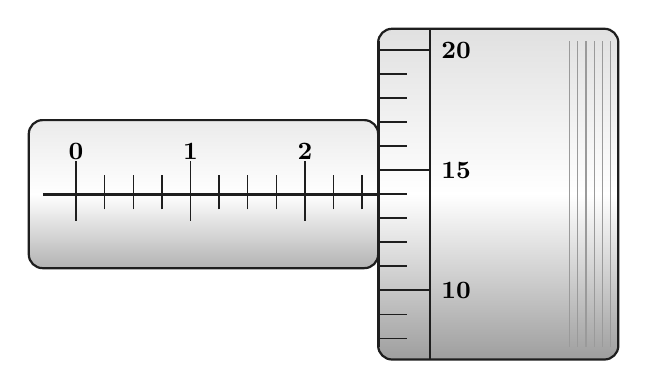
\begin{tikzpicture}[scale=1]
  \shade[rounded corners=5pt,top color=black!8,bottom color=black!30,middle color=white] (0,-0.94) rectangle (4.4372,0.94);
  \draw[scb,rounded corners=5pt] (0,-0.94) rectangle (4.4372,0.94);
  \draw[draw=figline,line width=1.1pt] (0.18,0) -- (4.4372,0);
  \draw[sc] (0.6,-0.336) -- (0.6,0.42);
  \node[lab,above] at (0.6,0.40) {0};
  \draw[sc] (0.9634,-0.192) -- (0.9634,0.24);
  \draw[sc] (1.3267,-0.192) -- (1.3267,0.24);
  \draw[sc] (1.6901,-0.192) -- (1.6901,0.24);
  \draw[sc] (2.0535,-0.336) -- (2.0535,0.42);
  \node[lab,above] at (2.0535,0.40) {1};
  \draw[sc] (2.4169,-0.192) -- (2.4169,0.24);
  \draw[sc] (2.7802,-0.192) -- (2.7802,0.24);
  \draw[sc] (3.1436,-0.192) -- (3.1436,0.24);
  \draw[sc] (3.507,-0.336) -- (3.507,0.42);
  \node[lab,above] at (3.507,0.40) {2};
  \draw[sc] (3.8703,-0.192) -- (3.8703,0.24);
  \draw[sc] (4.2337,-0.192) -- (4.2337,0.24);
  \shade[rounded corners=5pt,top color=black!12,bottom color=black!38,middle color=white] (4.4372,-2.1) rectangle (7.4872,2.1);
  \draw[scb,rounded corners=5pt] (4.4372,-2.1) rectangle (7.4872,2.1);
  \draw[draw=figline,line width=1.0pt] (4.4372,-1.94) -- (4.4372,1.94);
  \draw[sc] (5.0972,-2.1) -- (5.0972,2.1);
  \draw[draw=figline!45,line width=0.4pt] (6.8672,-1.94) -- (6.8672,1.94);
  \draw[draw=figline!45,line width=0.4pt] (6.9722,-1.94) -- (6.9722,1.94);
  \draw[draw=figline!45,line width=0.4pt] (7.0772,-1.94) -- (7.0772,1.94);
  \draw[draw=figline!45,line width=0.4pt] (7.1822,-1.94) -- (7.1822,1.94);
  \draw[draw=figline!45,line width=0.4pt] (7.2872,-1.94) -- (7.2872,1.94);
  \draw[draw=figline!45,line width=0.4pt] (7.3922,-1.94) -- (7.3922,1.94);
  \draw[draw=figline,line width=0.5pt] (4.4372,-1.83) -- (4.8002,-1.83);
  \draw[draw=figline,line width=0.5pt] (4.4372,-1.525) -- (4.8002,-1.525);
  \draw[draw=figline,line width=0.9pt] (4.4372,-1.22) -- (5.0972,-1.22);
  \node[lab,right] at (5.1972,-1.22) {10};
  \draw[draw=figline,line width=0.5pt] (4.4372,-0.915) -- (4.8002,-0.915);
  \draw[draw=figline,line width=0.5pt] (4.4372,-0.61) -- (4.8002,-0.61);
  \draw[draw=figline,line width=0.5pt] (4.4372,-0.305) -- (4.8002,-0.305);
  \draw[draw=figline,line width=0.5pt] (4.4372,0) -- (4.8002,0);
  \draw[draw=figline,line width=0.9pt] (4.4372,0.305) -- (5.0972,0.305);
  \node[lab,right] at (5.1972,0.305) {15};
  \draw[draw=figline,line width=0.5pt] (4.4372,0.61) -- (4.8002,0.61);
  \draw[draw=figline,line width=0.5pt] (4.4372,0.915) -- (4.8002,0.915);
  \draw[draw=figline,line width=0.5pt] (4.4372,1.22) -- (4.8002,1.22);
  \draw[draw=figline,line width=0.5pt] (4.4372,1.525) -- (4.8002,1.525);
  \draw[draw=figline,line width=0.9pt] (4.4372,1.83) -- (5.0972,1.83);
  \node[lab,right] at (5.1972,1.83) {20};
\end{tikzpicture}
}

\newcommand{\figQBI}{%
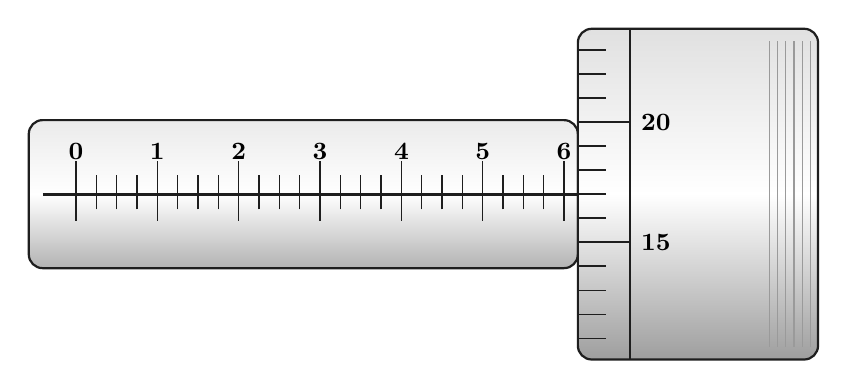
\begin{tikzpicture}[scale=1]
  \shade[rounded corners=5pt,top color=black!8,bottom color=black!30,middle color=white] (0,-0.94) rectangle (6.9736,0.94);
  \draw[scb,rounded corners=5pt] (0,-0.94) rectangle (6.9736,0.94);
  \draw[draw=figline,line width=1.1pt] (0.18,0) -- (6.9736,0);
  \draw[sc] (0.6,-0.336) -- (0.6,0.42);
  \node[lab,above] at (0.6,0.40) {0};
  \draw[sc] (0.8582,-0.192) -- (0.8582,0.24);
  \draw[sc] (1.1165,-0.192) -- (1.1165,0.24);
  \draw[sc] (1.3747,-0.192) -- (1.3747,0.24);
  \draw[sc] (1.633,-0.336) -- (1.633,0.42);
  \node[lab,above] at (1.633,0.40) {1};
  \draw[sc] (1.8912,-0.192) -- (1.8912,0.24);
  \draw[sc] (2.1495,-0.192) -- (2.1495,0.24);
  \draw[sc] (2.4077,-0.192) -- (2.4077,0.24);
  \draw[sc] (2.666,-0.336) -- (2.666,0.42);
  \node[lab,above] at (2.666,0.40) {2};
  \draw[sc] (2.9242,-0.192) -- (2.9242,0.24);
  \draw[sc] (3.1825,-0.192) -- (3.1825,0.24);
  \draw[sc] (3.4407,-0.192) -- (3.4407,0.24);
  \draw[sc] (3.699,-0.336) -- (3.699,0.42);
  \node[lab,above] at (3.699,0.40) {3};
  \draw[sc] (3.9572,-0.192) -- (3.9572,0.24);
  \draw[sc] (4.2155,-0.192) -- (4.2155,0.24);
  \draw[sc] (4.4737,-0.192) -- (4.4737,0.24);
  \draw[sc] (4.732,-0.336) -- (4.732,0.42);
  \node[lab,above] at (4.732,0.40) {4};
  \draw[sc] (4.9902,-0.192) -- (4.9902,0.24);
  \draw[sc] (5.2485,-0.192) -- (5.2485,0.24);
  \draw[sc] (5.5067,-0.192) -- (5.5067,0.24);
  \draw[sc] (5.765,-0.336) -- (5.765,0.42);
  \node[lab,above] at (5.765,0.40) {5};
  \draw[sc] (6.0232,-0.192) -- (6.0232,0.24);
  \draw[sc] (6.2815,-0.192) -- (6.2815,0.24);
  \draw[sc] (6.5397,-0.192) -- (6.5397,0.24);
  \draw[sc] (6.798,-0.336) -- (6.798,0.42);
  \node[lab,above] at (6.798,0.40) {6};
  \shade[rounded corners=5pt,top color=black!12,bottom color=black!38,middle color=white] (6.9736,-2.1) rectangle (10.0236,2.1);
  \draw[scb,rounded corners=5pt] (6.9736,-2.1) rectangle (10.0236,2.1);
  \draw[draw=figline,line width=1.0pt] (6.9736,-1.94) -- (6.9736,1.94);
  \draw[sc] (7.6336,-2.1) -- (7.6336,2.1);
  \draw[draw=figline!45,line width=0.4pt] (9.4036,-1.94) -- (9.4036,1.94);
  \draw[draw=figline!45,line width=0.4pt] (9.5086,-1.94) -- (9.5086,1.94);
  \draw[draw=figline!45,line width=0.4pt] (9.6136,-1.94) -- (9.6136,1.94);
  \draw[draw=figline!45,line width=0.4pt] (9.7186,-1.94) -- (9.7186,1.94);
  \draw[draw=figline!45,line width=0.4pt] (9.8236,-1.94) -- (9.8236,1.94);
  \draw[draw=figline!45,line width=0.4pt] (9.9286,-1.94) -- (9.9286,1.94);
  \draw[draw=figline,line width=0.5pt] (6.9736,-1.83) -- (7.3366,-1.83);
  \draw[draw=figline,line width=0.5pt] (6.9736,-1.525) -- (7.3366,-1.525);
  \draw[draw=figline,line width=0.5pt] (6.9736,-1.22) -- (7.3366,-1.22);
  \draw[draw=figline,line width=0.5pt] (6.9736,-0.915) -- (7.3366,-0.915);
  \draw[draw=figline,line width=0.9pt] (6.9736,-0.61) -- (7.6336,-0.61);
  \node[lab,right] at (7.7336,-0.61) {15};
  \draw[draw=figline,line width=0.5pt] (6.9736,-0.305) -- (7.3366,-0.305);
  \draw[draw=figline,line width=0.5pt] (6.9736,0) -- (7.3366,0);
  \draw[draw=figline,line width=0.5pt] (6.9736,0.305) -- (7.3366,0.305);
  \draw[draw=figline,line width=0.5pt] (6.9736,0.61) -- (7.3366,0.61);
  \draw[draw=figline,line width=0.9pt] (6.9736,0.915) -- (7.6336,0.915);
  \node[lab,right] at (7.7336,0.915) {20};
  \draw[draw=figline,line width=0.5pt] (6.9736,1.22) -- (7.3366,1.22);
  \draw[draw=figline,line width=0.5pt] (6.9736,1.525) -- (7.3366,1.525);
  \draw[draw=figline,line width=0.5pt] (6.9736,1.83) -- (7.3366,1.83);
\end{tikzpicture}
}


\begin{document}

\begin{center}
  {\LARGE\bfseries EnergyTech}\\[2pt]
  {\Large Chapter 04 --- Version B}\\[6pt]
  Name: \rule{4.5cm}{0.4pt}\quad Group: \rule{3cm}{0.4pt}\quad SPSP ID: \rule{3.5cm}{0.4pt}
\end{center}

\begin{multicols}{2}
\raggedcolumns
% ---------------- Q1 ----------------
\begin{Qbox}{1}{4-1.1}
Determine the accuracy of the measurement; that is, give the number of significant digits for the measurement.\par\medskip $42{,}500$ kg
\begin{choices}
  \item 2
  \item 5
  \item 4
  \item 3
\end{choices}
\qrcode[height=2.2cm,hyperlink]{https://www.youtube.com/watch?v=FhLOHZ4jlP8}
\end{Qbox}

% ---------------- Q2 ----------------
\begin{Qbox}{2}{4-1.1}
Determine the accuracy of the measurement; that is, give the number of significant digits for the measurement.\par\medskip $607{,}3\overline{0}0$
\begin{choices}
  \item 5
  \item 4
  \item 6
  \item 7
\end{choices}
\qrcode[height=2.2cm,hyperlink]{https://www.youtube.com/watch?v=O2WRBUsIeZc}
\end{Qbox}

% ---------------- Q3 ----------------
\begin{Qbox}{3}{4-1.1}
Determine the accuracy of the measurement; that is, give the number of significant digits for the measurement.\par\medskip $0.0060$ g
\begin{choices}
  \item 2
  \item 1
  \item 3
  \item 5
\end{choices}
\qrcode[height=2.2cm,hyperlink]{https://www.youtube.com/watch?v=29VCgAWuS08}
\end{Qbox}

% ---------------- Q4 ----------------
\begin{Qbox}{4}{4-1.1}
Determine the accuracy of the measurement; that is, give the number of significant digits for the measurement.\par\medskip $0.0483000$ A
\begin{choices}
  \item 5
  \item 7
  \item 6
  \item 8
\end{choices}
\qrcode[height=2.2cm,hyperlink]{https://www.youtube.com/watch?v=gEq2wwiqNB8}
\end{Qbox}

% ---------------- Q5 ----------------
\begin{Qbox}{5}{4-1.1}
Determine the accuracy of the measurement; that is, give the number of significant digits for the measurement.\par\medskip $2{,}936$ m
\begin{choices}
  \item 3
  \item 6
  \item 5
  \item 4
\end{choices}
\qrcode[height=2.2cm,hyperlink]{https://www.youtube.com/watch?v=_FD3dS7Vg3U}
\end{Qbox}

% ---------------- Q6 ----------------
\begin{Qbox}{6}{4-1.1}
Determine the accuracy of the measurement; that is, give the number of significant digits for the measurement.\par\medskip $728{,}400$ g
\begin{choices}
  \item 4
  \item 5
  \item 6
  \item 3
\end{choices}
\qrcode[height=2.2cm,hyperlink]{https://www.youtube.com/watch?v=NZMZXixpuv4}
\end{Qbox}

% ---------------- Q7 ----------------
\begin{Qbox}{7}{4-2.1}
The measurement is 8.2500 A. Find the precision.
\begin{choices}
  \item The precision of the measurement is 0.00001 A
  \item The precision of the measurement is 0.000001 A
  \item The precision of the measurement is 0.0001 A
  \item The precision of the measurement is 0.001 A
\end{choices}
\qrcode[height=2.2cm,hyperlink]{https://www.youtube.com/watch?v=xKxx56lye3g}
\end{Qbox}

% ---------------- Q8 ----------------
\begin{Qbox}{8}{4-2.1}
The measurement is 145.0 cm. Find the precision.
\begin{choices}
  \item The precision is 0.001 cm
  \item The precision is 0.01 cm
  \item The precision is 1 cm
  \item The precision is 0.1 cm
\end{choices}
\qrcode[height=2.2cm,hyperlink]{https://www.youtube.com/watch?v=1JnWFd0IspY}
\end{Qbox}

% ---------------- Q9 ----------------
\begin{Qbox}{9}{4-2.1}
The measurement is 6.000 in. Find the precision.
\begin{choices}
  \item The precision is 0.01 in
  \item The precision is 0.00001 in
  \item The precision is 0.001 in
  \item The precision is 0.0001 in
\end{choices}
\qrcode[height=2.2cm,hyperlink]{https://www.youtube.com/watch?v=kZ6FfJt_LTA}
\end{Qbox}

% ---------------- Q10 ----------------
\begin{Qbox}{10}{4-2.1}
The measurement is 872 km. Find the precision.
\begin{choices}
  \item The precision is 0.01 km
  \item The precision is 1 km
  \item The precision is 0.1 km
  \item The precision is 10 km
\end{choices}
\qrcode[height=2.2cm,hyperlink]{https://www.youtube.com/watch?v=Uptz7jfWnVI}
\end{Qbox}

% ---------------- Q11 ----------------
\begin{Qbox}{11}{4-2.1}
The measurement is $68{,}\overline{0}00$ km. Find the precision.
\begin{choices}
  \item The precision is 10 km
  \item The precision is 100 km
  \item The precision is 1 km
  \item The precision is 1000 km
\end{choices}
\qrcode[height=2.2cm,hyperlink]{https://www.youtube.com/watch?v=SE7YQtbcBeg}
\end{Qbox}

% ---------------- Q12 ----------------
\begin{Qbox}{12}{4-2.1}
The measurement is 73.20400 mi. Find the precision.
\begin{choices}
  \item The precision is 0.00001 mi
  \item The precision is 0.000001 mi
  \item The precision is 0.0000001 mi
  \item The precision is 0.0001 mi
\end{choices}
\qrcode[height=2.2cm,hyperlink]{https://www.youtube.com/watch?v=cksn4vK3mhk}
\end{Qbox}

% ---------------- Q13 ----------------
\begin{Qbox}{13}{4-2.2}
The measurement is 7.2840 cm. Find the greatest possible error of the measurement.
\begin{choices}
  \item The greatest possible error is 0.0005 cm
  \item The greatest possible error is 0.0001 cm
  \item The greatest possible error is 0.00005 cm
  \item The greatest possible error is 0.000005 cm
\end{choices}
\qrcode[height=2.2cm,hyperlink]{https://www.youtube.com/watch?v=L-TsjdvD7ZQ}
\end{Qbox}

% ---------------- Q14 ----------------
\begin{Qbox}{14}{4-2.2}
The measurement is 45.610 m. Find the greatest possible error of the measurement.
\begin{choices}
  \item The greatest possible error is 0.0005 m
  \item The greatest possible error is 0.001 m
  \item The greatest possible error is 0.00005 m
  \item The greatest possible error is 0.005 m
\end{choices}
\qrcode[height=2.2cm,hyperlink]{https://www.youtube.com/watch?v=QKBMWpAA95s}
\end{Qbox}

% ---------------- Q15 ----------------
\begin{Qbox}{15}{4-2.2}
The measurement is 9.15 m. Find the greatest possible error of the measurement.
\begin{choices}
  \item The greatest possible error is 0.01 m
  \item The greatest possible error is 0.005 m
  \item The greatest possible error is 0.0005 m
  \item The greatest possible error is 0.05 m
\end{choices}
\qrcode[height=2.2cm,hyperlink]{https://www.youtube.com/watch?v=7kzsFh5ax-8}
\end{Qbox}

% ---------------- Q16 ----------------
\begin{Qbox}{16}{4-2.1 / 4-2.2}
The measurement is $21\frac{7}{16}$ in. Find the precision and the greatest possible error of the measurement.
\begin{choices}
  \item Precision $=\dfrac{1}{16}$, greatest possible error $=\dfrac{1}{32}$
  \item Precision $=\dfrac{1}{32}$, greatest possible error $=\dfrac{1}{16}$
  \item Precision $=\dfrac{1}{32}$, greatest possible error $=\dfrac{1}{32}$
  \item Precision $=\dfrac{1}{16}$, greatest possible error $=\dfrac{1}{16}$
\end{choices}
\qrcode[height=2.2cm,hyperlink]{https://www.youtube.com/watch?v=FbGULnhUr58}
\end{Qbox}

% ---------------- Q17 ----------------
\begin{Qbox}{17}{4-2.1 / 4-2.2}
The measurement is $5\frac{9}{20}$ in. Find the precision and the greatest possible error of the measurement.
\begin{choices}
  \item Precision $=\dfrac{1}{40}$, greatest possible error $=\dfrac{1}{40}$
  \item Precision $=\dfrac{1}{40}$, greatest possible error $=\dfrac{1}{20}$
  \item Precision $=\dfrac{1}{20}$, greatest possible error $=\dfrac{1}{20}$
  \item Precision $=\dfrac{1}{20}$, greatest possible error $=\dfrac{1}{40}$
\end{choices}
\qrcode[height=2.2cm,hyperlink]{https://www.youtube.com/watch?v=8v8T6GLrV7M}
\end{Qbox}

% ---------------- Q18 ----------------
\begin{Qbox}{18}{4-3.1}
In the given Vernier Caliper, part I is \ldots
\incfig{210}{fig_caliper.png}
\begin{choices}
  \item Jaws
  \item Beam
  \item Depth gauge
  \item Small jaws
\end{choices}
\qrcode[height=2.2cm,hyperlink]{https://www.youtube.com/watch?v=CKAhOUBv_Ck}
\end{Qbox}

% ---------------- Q19 ----------------
\begin{Qbox}{19}{4-3.1}
In the given Vernier Caliper, part K is \ldots
\incfig{210}{fig_caliper.png}
\begin{choices}
  \item Metric Vernier scale
  \item U.S. Fixed scale
  \item Metric Fixed scale
  \item U.S. Vernier scale
\end{choices}
\qrcode[height=2.2cm,hyperlink]{https://www.youtube.com/watch?v=eydw_enMeQk}
\end{Qbox}

% ---------------- Q20 ----------------
\begin{Qbox}{20}{4-3.1}
Read the measurement in millimeter shown on the vernier caliper.
\figbox{\figQBZ}
\begin{choices}
  \item 1.472 mm
  \item 37.40 mm
  \item 1.427 mm
  \item 37.04 mm
\end{choices}
\qrcode[height=2.2cm,hyperlink]{https://www.youtube.com/watch?v=m5Lp71cWcFE}
\end{Qbox}

% ---------------- Q21 ----------------
\begin{Qbox}{21}{4-3.2}
Read the measurement in millimeter shown on the vernier caliper.
\figbox{\figQBA}
\begin{choices}
  \item 3.648 mm
  \item 3.684 mm
  \item 92.56 mm
  \item 92.65 mm
\end{choices}
\qrcode[height=2.2cm,hyperlink]{https://www.youtube.com/watch?v=xVg0hxrQ4Jg}
\end{Qbox}

% ---------------- Q22 ----------------
\begin{Qbox}{22}{4-3.3}
Read the measurement in inch shown on the vernier caliper.
\figbox{\figQBB}
\begin{choices}
  \item 1.874 in
  \item 1.847 in
  \item 0.847 in
  \item 46.90 in
\end{choices}
\qrcode[height=2.2cm,hyperlink]{https://www.youtube.com/watch?v=wcmLZgkqi3M}
\end{Qbox}

% ---------------- Q23 ----------------
\begin{Qbox}{23}{4-3.3}
Read the measurement in inch shown on the vernier caliper.
\figbox{\figQBC}
\begin{choices}
  \item 2.536 in
  \item 65.10 in
  \item 0.563 in
  \item 2.563 in
\end{choices}
\qrcode[height=2.2cm,hyperlink]{https://www.youtube.com/watch?v=bXo3POT01eE}
\end{Qbox}

% ---------------- Q24 ----------------
\begin{Qbox}{24}{4-4.1}
In the given Micrometer Caliper, part G is
\incfig{200}{fig_micrometer.png}
\begin{choices}
  \item Spindle
  \item Thimble
  \item Anvil
  \item Ratchet
\end{choices}
\qrcode[height=2.2cm,hyperlink]{https://www.youtube.com/watch?v=0XkBVkZvfvA}
\end{Qbox}

% ---------------- Q25 ----------------
\begin{Qbox}{25}{4-4.1}
In the given Micrometer Caliper, part F is
\incfig{200}{fig_micrometer.png}
\begin{choices}
  \item Spindle
  \item Ratchet
  \item Anvil
  \item Thimble
\end{choices}
\qrcode[height=2.2cm,hyperlink]{https://www.youtube.com/watch?v=89Bz6HZpME8}
\end{Qbox}

% ---------------- Q26 ----------------
\begin{Qbox}{26}{4-4.2}
Read the measurement shown on the metric micrometer.
\figbox{\figQBF}
\begin{choices}
  \item 42.8 mm
  \item 4.27 mm
  \item 4.28 mm
  \item 4.29 mm
\end{choices}
\qrcode[height=2.2cm,hyperlink]{https://www.youtube.com/watch?v=n0lpdXKX8NA}
\end{Qbox}

% ---------------- Q27 ----------------
\begin{Qbox}{27}{4-4.2}
Read the measurement shown on the metric micrometer.
\figbox{\figQBG}
\begin{choices}
  \item 12.65 mm
  \item 12.66 mm
  \item 126.5 mm
  \item 12.15 mm
\end{choices}
\qrcode[height=2.2cm,hyperlink]{https://www.youtube.com/watch?v=MplthM6FZQU}
\end{Qbox}

% ---------------- Q28 ----------------
\begin{Qbox}{28}{4-4.4}
Read the measurement shown on the U.S. micrometer.
\figbox{\figQBH}
\begin{choices}
  \item 2.640 in
  \item 0.250 in
  \item 0.289 in
  \item 0.264 in
\end{choices}
\qrcode[height=2.2cm,hyperlink]{https://www.youtube.com/watch?v=tTfhEPs7AG4}
\end{Qbox}

% ---------------- Q29 ----------------
\begin{Qbox}{29}{4-4.3}
Read the measurement shown on the U.S. micrometer.
\figbox{\figQBI}
\begin{choices}
  \item 0.617 in
  \item 0.642 in
  \item 0.600 in
  \item 6.170 in
\end{choices}
\qrcode[height=2.2cm,hyperlink]{https://www.youtube.com/watch?v=BSleiTcnV88}
\end{Qbox}

% ---------------- Q30 ----------------
\begin{Qbox}{30}{4-5.1}
Find the measurement that is the most accurate.
\begin{choices}
  \item 742 ft
  \item 400 ft
  \item 950 ft
  \item 3,600 ft
\end{choices}
\qrcode[height=2.2cm,hyperlink]{https://www.youtube.com/watch?v=wFtUtuKgrnI}
\end{Qbox}

% ---------------- Q31 ----------------
\begin{Qbox}{31}{4-5.1}
Find the measurement that is the most accurate.
\begin{choices}
  \item 806 ft
  \item 240 ft
  \item 900 ft
  \item 1,500 ft
\end{choices}
\qrcode[height=2.2cm,hyperlink]{https://www.youtube.com/watch?v=fi2FP7z8XXk}
\end{Qbox}

% ---------------- Q32 ----------------
\begin{Qbox}{32}{4-5.1}
Find the measurement that is the most accurate.
\begin{choices}
  \item 683 ft
  \item 2,700 ft
  \item 500 ft
  \item 370 ft
\end{choices}
\qrcode[height=2.2cm,hyperlink]{https://www.youtube.com/watch?v=S8T8OfIpWdU}
\end{Qbox}

% ---------------- Q33 ----------------
\begin{Qbox}{33}{4-5.1}
Find the measurement that is the most accurate.
\begin{choices}
  \item 3400 ft
  \item 0.7600 ft
  \item 7000 ft
  \item 0.00410 ft
\end{choices}
\qrcode[height=2.2cm,hyperlink]{https://www.youtube.com/watch?v=kmIhRWkySiY}
\end{Qbox}

% ---------------- Q34 ----------------
\begin{Qbox}{34}{4-5.1}
Find the measurement that is the least accurate.
\begin{choices}
  \item 22.4000 in
  \item 0.000740 in
  \item 0.00060 in
  \item 5000 in
\end{choices}
\qrcode[height=2.2cm,hyperlink]{https://www.youtube.com/watch?v=i50ZER16Vic}
\end{Qbox}

% ---------------- Q35 ----------------
\begin{Qbox}{35}{4-5.1}
Find the measurement that is the least accurate.
\begin{choices}
  \item 2340000 m
  \item 260000 m
  \item 47200 m
  \item 0.00730 m
\end{choices}
\qrcode[height=2.2cm,hyperlink]{https://www.youtube.com/watch?v=M7AB8u72_8k}
\end{Qbox}

% ---------------- Q36 ----------------
\begin{Qbox}{36}{4-5.1}
Find the measurement that is the least accurate.
\begin{choices}
  \item 71.0000 in
  \item 45000 in
  \item 3000 in
  \item 0.000560 in
\end{choices}
\qrcode[height=2.2cm,hyperlink]{https://www.youtube.com/watch?v=d32PX6zaUhM}
\end{Qbox}

% ---------------- Q37 ----------------
\begin{Qbox}{37}{4-5.1}
Find the measurement that is the most accurate.
\begin{choices}
  \item 0.075 A
  \item 0.074 A
  \item 0.0880 A
  \item 0.00050 A
\end{choices}
\qrcode[height=2.2cm,hyperlink]{https://www.youtube.com/watch?v=kfDJ24QBcuI}
\end{Qbox}

% ---------------- Q38 ----------------
\begin{Qbox}{38}{4-5.1}
Find the measurement that is the least accurate.
\begin{choices}
  \item 52,000 V
  \item 60,000 V
  \item 41,000 V
  \item 3,400,000 V
\end{choices}
\qrcode[height=2.2cm,hyperlink]{https://www.youtube.com/watch?v=CdvPb7S0h9Y}
\end{Qbox}

% ---------------- Q39 ----------------
\begin{Qbox}{39}{4-5.1}
Find the measurement that is the least accurate.
\begin{choices}
  \item 9,200 V
  \item 5,700,000 V
  \item 40,000 V
  \item 38,000 V
\end{choices}
\qrcode[height=2.2cm,hyperlink]{https://www.youtube.com/watch?v=mdd_74Yj1iA}
\end{Qbox}

% ---------------- Q40 ----------------
\begin{Qbox}{40}{4-5.1}
Find the measurement that is the least accurate.
\begin{choices}
  \item 0.0027 V
  \item 21,600 V
  \item 46.00 V
  \item 0.00930 V
\end{choices}
\qrcode[height=2.2cm,hyperlink]{https://www.youtube.com/watch?v=L0pMHrjqsEg}
\end{Qbox}

% ---------------- Q41 ----------------
\begin{Qbox}{41}{4-5.1}
Find the measurement that is the least accurate.
\begin{choices}
  \item 6.30000 ft
  \item 7.240 ft
  \item 0.3600 ft
  \item 84,000 ft
\end{choices}
\qrcode[height=2.2cm,hyperlink]{https://www.youtube.com/watch?v=nQ0DitEi1Ps}
\end{Qbox}

% ---------------- Q42 ----------------
\begin{Qbox}{42}{4-5.1}
Find the measurement that is the least accurate.
\begin{choices}
  \item 700 ft
  \item 673 ft
  \item 880 ft
  \item 604 ft
\end{choices}
\qrcode[height=2.2cm,hyperlink]{https://www.youtube.com/watch?v=Y1cHxGjrkjU}
\end{Qbox}

% ---------------- Q43 ----------------
\begin{Qbox}{43}{4-5.1}
Find the measurement that is the least accurate.
\begin{choices}
  \item 760 ft
  \item 500 ft
  \item 815 ft
  \item 837 ft
\end{choices}
\qrcode[height=2.2cm,hyperlink]{https://www.youtube.com/watch?v=eBSkNlhA6Wc}
\end{Qbox}

% ---------------- Q44 ----------------
\begin{Qbox}{44}{4-5.1}
Find the measurement that is the least accurate.
\begin{choices}
  \item 400 ft
  \item 508 ft
  \item 534 ft
  \item 630 ft
\end{choices}
\qrcode[height=2.2cm,hyperlink]{https://www.youtube.com/watch?v=toC9PYl0yHk}
\end{Qbox}

% ---------------- Q45 ----------------
\begin{Qbox}{45}{4-5.1}
Use the rules of measurements to evaluate.\par\medskip $(4{,}200\ \text{cm})(27.00\ \text{cm})$
\begin{choices}
  \item 100,000 cm$^2$
  \item 110,000 cm$^2$
  \item 113,000 cm$^2$
  \item 113,400 cm$^2$
\end{choices}
\qrcode[height=2.2cm,hyperlink]{https://www.youtube.com/watch?v=_Xjo5E_pcYo}
\end{Qbox}

% ---------------- Q46 ----------------
\begin{Qbox}{46}{4-6.1}
Use the rules of measurements to evaluate.\par\medskip $(3{,}600\ \text{m})(70\ \text{m})(1450\ \text{m})$
\begin{choices}
  \item 400,000,000 m$^3$
  \item 365,400,000 m$^3$
  \item 370,000,000 m$^3$
  \item 365,000,000 m$^3$
\end{choices}
\qrcode[height=2.2cm,hyperlink]{https://www.youtube.com/watch?v=vd7Sg-5mZc0}
\end{Qbox}

% ---------------- Q47 ----------------
\begin{Qbox}{47}{4-6.1}
Use the rules of measurements to evaluate.\par\medskip $74{,}600$ V $\div\ 2.8$ A
\begin{choices}
  \item 30,000 V/A
  \item 27,000 V/A
  \item 26,600 V/A
  \item 26,643 V/A
\end{choices}
\qrcode[height=2.2cm,hyperlink]{https://www.youtube.com/watch?v=rLAH-4JSDRo}
\end{Qbox}

% ---------------- Q48 ----------------
\begin{Qbox}{48}{4-6.1}
Use the rules of measurements to evaluate.\[ \frac{(4180\ m)(3.5\ L)}{4.0\ s} \]
\begin{choices}
  \item $4{,}000\ mL/s$
  \item $3{,}700\ mL/s$
  \item $3.700\ mL/s$
  \item $3{,}658\ mL/s$
\end{choices}
\qrcode[height=2.2cm,hyperlink]{https://www.youtube.com/watch?v=rGtejzjn64U}
\end{Qbox}

% ---------------- Q49 ----------------
\begin{Qbox}{49}{4-6.1}
Find the area of a rectangle 3.40 cm by 61.0 cm. $(A=l\cdot w)$ (Use the rules for working with measurements).
\begin{choices}
  \item 207.4 cm$^2$
  \item 207 cm$^2$
  \item 200 cm$^2$
  \item 210 cm$^2$
\end{choices}
\qrcode[height=2.2cm,hyperlink]{https://www.youtube.com/watch?v=OVOHkqfkrEI}
\end{Qbox}

% ---------------- Q50 ----------------
\begin{Qbox}{50}{4-6.1}
Find the volume of a rectangular solid when $l=3.50$ ft, $w=6.0$ ft, and $h=41.40$ ft.\par\medskip $V=lwh$, where $l$ length, $w$ width, and $h$ height.\par\medskip (Use the rules for working with measurements)
\begin{choices}
  \item 869.4 ft$^3$
  \item 900 ft$^3$
  \item 869 ft$^3$
  \item 870 ft$^3$
\end{choices}
\qrcode[height=2.2cm,hyperlink]{https://www.youtube.com/watch?v=6P8cDZvSm3M}
\end{Qbox}

\end{multicols}
\end{document}
